\documentclass[crop,tikz]{standalone}
\usepackage{pgfplots}
\usepackage{amsmath}

\usetikzlibrary{decorations.markings}

\tikzset{%
    >=latex,% default arrow style
    ->-/.style={postaction={decorate},decoration={%
            markings,mark=at position #1 with {\arrow{>}}%
        }%
    },%
    ->-/.default=.5,%
    -<-/.style={postaction={decorate},decoration={%
            markings,mark=at position #1 with {\arrowreversed{>}}%
        }%
    },%
    -<-/.default=.5%
}

\pgfplotsset{
  compat=1.16,
  inverted/.style = {
    every axis legend/.append style={
      draw=white,
      fill=hardblack,
      text=white
    }
  },
  every non boxed x axis/.append style={
    axis line style={-latex}
  },
  every non boxed y axis/.append style={
    axis line style={-latex}
  },
  every non boxed z axis/.append style={
    axis line style={-latex}
  },
  /pgf/number format/.cd, use comma, 1000 sep={\,}
  % every boxed x axis/.style={}
}

\begin{document}
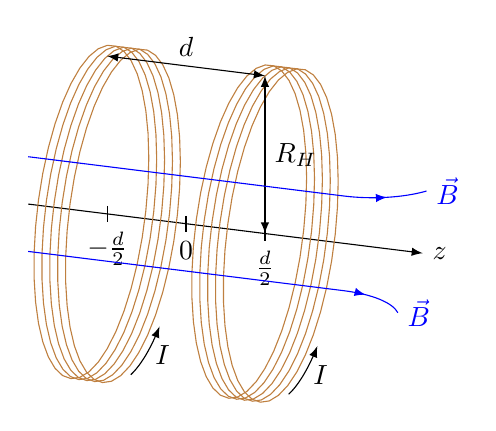
\begin{tikzpicture}
  \begin{axis}[
    width=0.8\textwidth,
    view={20}{20},
    axis equal image,
    axis lines=middle,
    y axis line style={draw=none},
    z axis line style={draw=none},
    xtick={\empty},
    xticklabels={\empty},
    ytick={\empty},
    yticklabels={\empty},
    ztick={\empty},
    zticklabels={\empty},
    xlabel={$z$},
    xlabel style={anchor=west},
    xmin=-1,xmax=1.5,
    ymin=-1,ymax=1,
    zmin=-1,zmax=1,
    samples=40,
    ]
    \pgfplotsinvokeforeach{-0.1,-0.05,...,0.1}{
      \addplot3[brown,variable=t,domain=0:{2*pi}] ({-0.5+#1},{cos(deg(t))},{sin(deg(t))});
      \addplot3[brown,variable=t,domain=0:{2*pi}] ({+0.5+#1},{cos(deg(t))},{sin(deg(t))});
    }
    \draw (-0.5,0,0.05) -- (-0.5,0,-0.05) node[below] {$-\frac{d}{2}$};
    \draw (   0,0,0.05) -- (   0,0,-0.05) node[below] {$0$};
    \draw (+0.5,0,0.05) -- (+0.5,0,-0.05) node[below] {$\frac{d}{2}$};
    \draw[<->] (0.5,0,0) -- node[right] {$R_H$} (0.5,0,1);
    \draw[<->] (-0.5,0,1) -- node[above] {$d$} (0.5,0,1);
    % current
    \pgfplotsinvokeforeach{-0.5,0.5}{
      \addplot3[->,variable=t,domain={3*pi/2}:{3*pi/2+pi/6},samples y=0] ({#1+0.15},{cos(deg(t))},{sin(deg(t))}) node[pos=0.5,right] {$I$};
    }
    % magnetic field
    \draw[blue,->-=0.9] (-1,0,+0.3) -- (1,0,+0.3) arc (270:330:0.5) node[right] {$\vec{B}$};
    \draw[blue,->-=0.9] (-1,0,-0.3) -- (1,0,-0.3) arc (90:30:0.5) node[right] {$\vec{B}$};
  \end{axis}
\end{tikzpicture}
\end{document}
